\subsection[Wykrywalność]{Wykrywalność}
\label{subsec:wykrywalnoscMK}
Po podłączeniu i uruchomieniu urządzenia system \textit{Windows 10} informuje użytkownika komunikatem ostrzegawczym o nierozpoznanym urządzeniu. Ostrzeżenie przedstawia rysunek~\ref{fig:windows1}.
Wykorzystana możliwość konfiguracji gadżetu USB w czasie wykonywania programu może skutkować chwilową błędną identyfikacją urządzenia przez system operacyjny.
W rezultacie użytkownik zostanie poinformowany stosownym komunikatem.
W przypadku przypadku realnego ataku, może to stanowić sygnał do sprawdzenia podłączonych urządzeń USB.
Osoba zaawansowana technicznie może skorzystać z narzędzi administracyjnych dostarczonych przez system operacyjny w celu zlokalizowania i zdiagnozowania przyczyny ostrzeżenia.
Przykładowy widok z panelu administracyjnego przedstawia rysunek~\ref{fig:windows2}.
\begin{figure}[H]
    \centering
    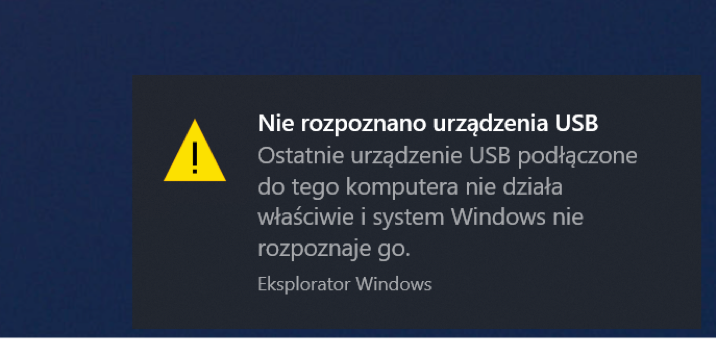
\includegraphics[width=0.8\textwidth]{mk03}
    \caption{Ostrzeżenie - nierozpoznane urządzenie}
    \label{fig:windows1}    
\end{figure}
\begin{figure}[H]
    \centering
    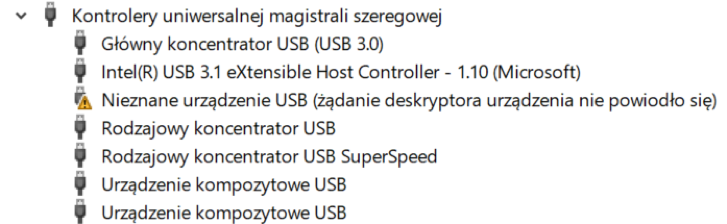
\includegraphics[width=\textwidth]{mk04}
    \caption{Fragment widoku panelu administracyjnego}
    \label{fig:windows2}    
\end{figure}